%第2章:準備


本章では,本論文で使用する用語,研究方針のフロー,商品識別システムの概要について述べる.

\section{諸定義}


\subsection*{V字モデル}

V字モデルとはソフトウェアの開発と確認の流れを模式的に示したものである.以下の図\ref{vji}にV字モデルの開発プロセスを示す.横軸は開発の時間軸であり,縦軸は詳細化の程度を表している\cite{kumikomi}.図\ref{vji}からもわかるように,詳細設計は単体テスト,基本設計は結合テストによって,要求分析は総合テストによって検証する.また,逆にテスト段階で判明した不具合は,左側の対応する設計にさかのぼった作業を必要とする\cite{soft}.本研究ではプロセスモデルとしてV字モデルを採用した.

\begin{figure}[htbp]
\centering
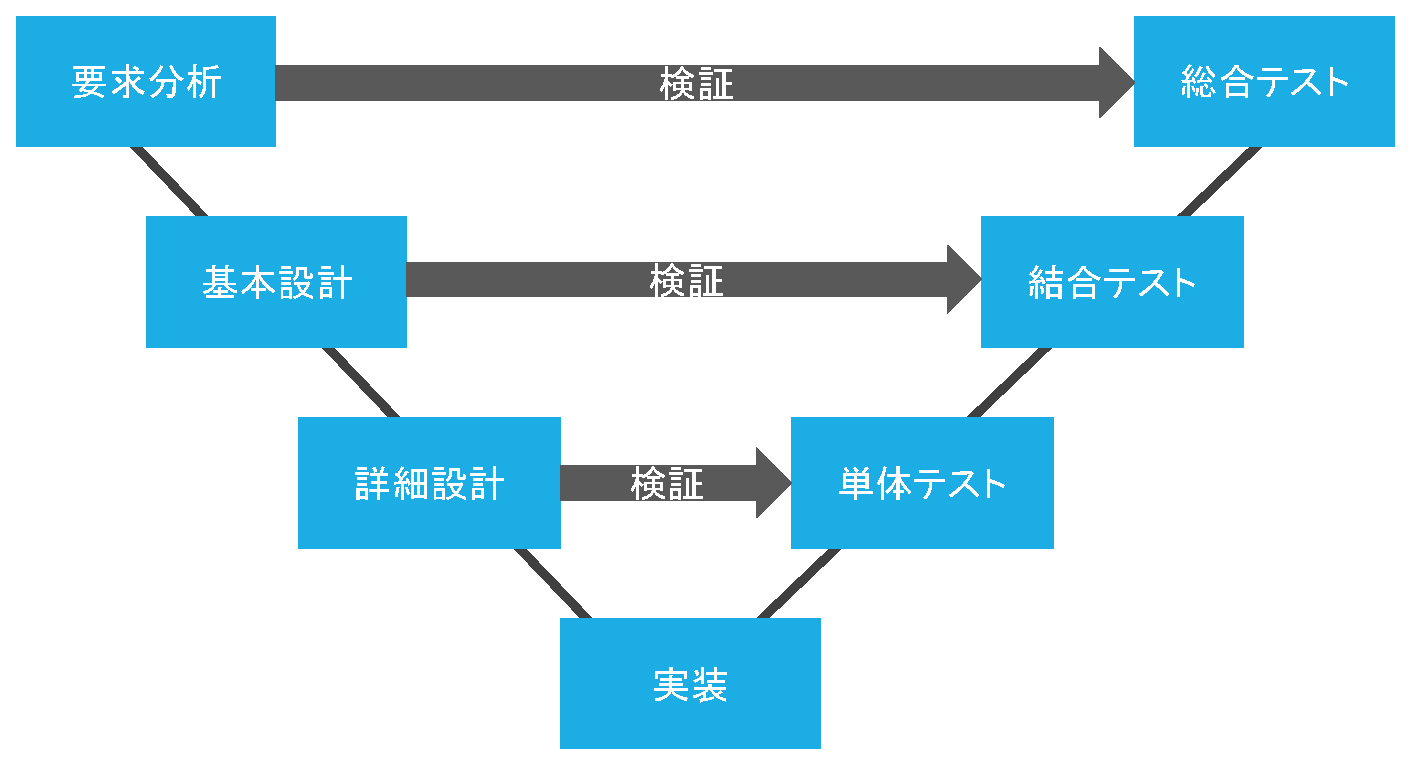
\includegraphics[width=12cm]{./picture/vjimodel.eps}
\caption{V字開発モデル}
\label{vji}
\end{figure}


\subsection*{UML(Unifiled Modeling Language)}

UMLとは統一モデリング言語(Unified Modeling Language)のことで,ビジネスや各種システムを対象としてその構造とダイナミクス(動的な振る舞いや挙動)をわかりやすく表現するためのビジュアルな言語\cite{uml}である.UMLの導入により,下記のような効用がもたらされる\cite{uml}.

\begin{itemize}
\item ユーザと開発者,または開発者どうしのコミュニケーションギャップの解消.
\item ユーザ要求の把握が正確になることで,仕様の認識違いによる出戻りの削減.
\item UMLによるオブジェクト指向設計が効果的にモジュール化を促進し,保守コストを削減.
\end{itemize}

\subsection*{ユースケース図}

ユーザの視点でシステムの機能的な流れを記述する記述法\cite{soft}であり,システムの使用イメージを表現する.システムがどのように機能すべきかという振る舞い(ユースケース)と,その外部環境(アクター)を表す.ユーザやクライアントの要求事項,システムに対して課せられている基本機能やサービス項目などの要件定義を表現するときに広く用いられる\cite{uml}.

\subsection*{クラス図}

システムをデータの視点から記述する図法\cite{soft}であり,システムが扱う情報構造を表す.問題領域の構造や対象システムの静的な構成,システムの詳細設計,あるいは企業の部門の業務モデルの基本構造,問題解決の最初のとっかかりとなる概念マップの構築,といったことに広く使\cite{uml}うことができる.

\subsection*{シーケンス図}

システムの一機能を実行の視点から記述する図法\cite{soft}	であり,システム機能がオブジェクトのメッセージのやり取りによってどのように達成されるかを示す.オブジェクト間のメッセージのやりとりを時系列に沿って並べて表現したもの\cite{uml}がシーケンス図である.


\section{商品識別システムの概要}

商品識別システムでは,WebカメラとRaspberry Pi,各種センサを各買い物カゴに設置し,従来のセルフレジやセミセルフレジに比べて安価かつ簡単に決済できる買い物を提案する.本システムの流れを図\ref{summary1}に示す.


\begin{figure}[htbp]
\centering
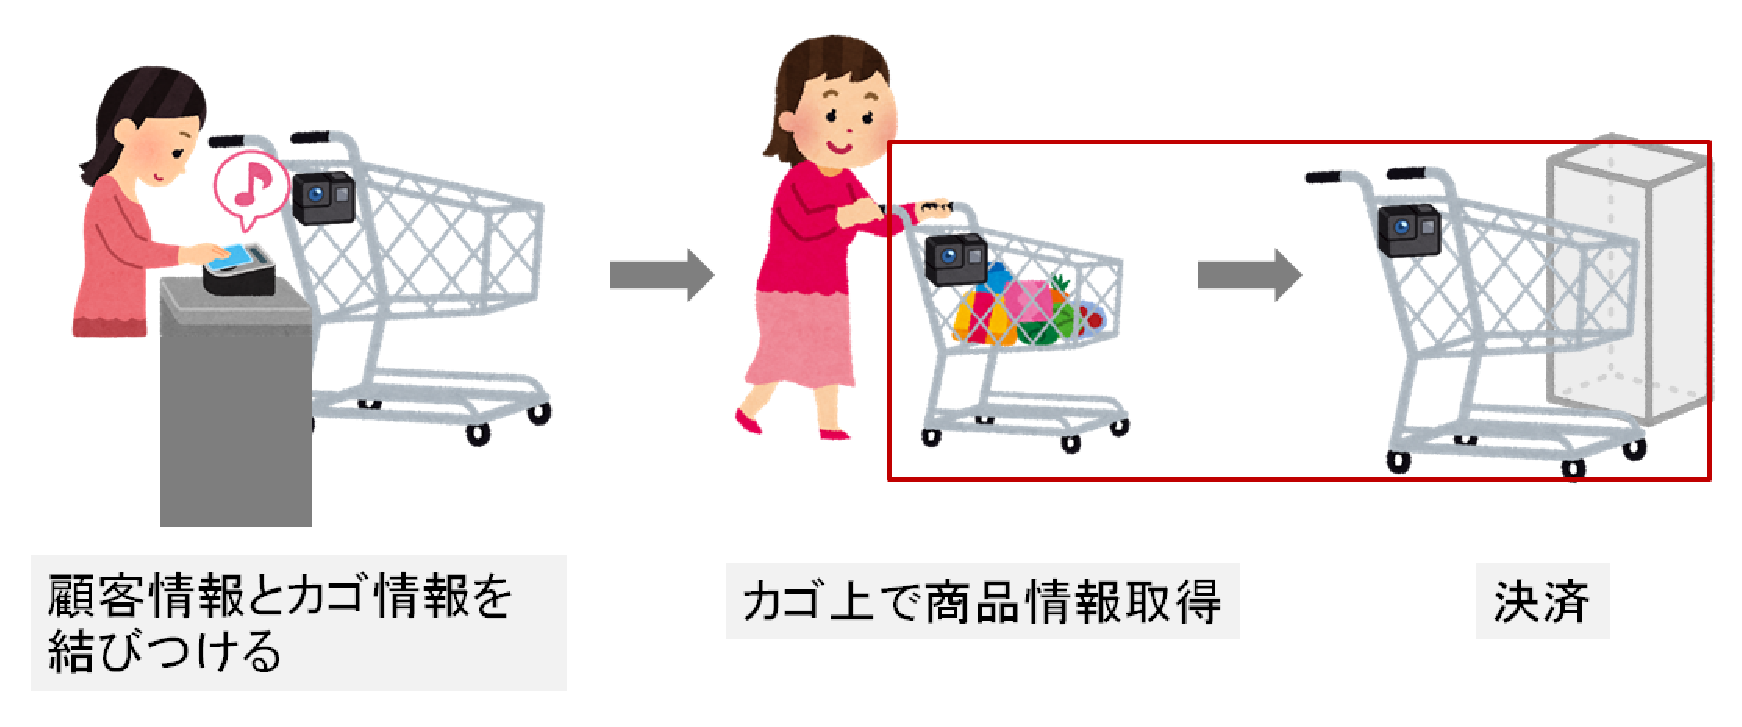
\includegraphics[width = 15cm]{./picture/summary1.eps}
\caption{商品識別システム全体の流れ}
\label{summary1}
\end{figure}



まず,顧客情報をカゴ情報と結び付ける.その後顧客はカゴに通常通り商品を入れる.その際,センシング技術を用いカゴ上で商品情報を取得しサーバへ情報を送信する.買い物を終える際は,カゴを返却するだけで決済が行われる流れとなる.本論文では図\ref{summary1}にある赤枠の範囲である,カゴ上で商品情報を取得し決済を行う部分を開発対象とした.本論文ではシステム全体の流れとシステム内上記の範囲を商品識別システムと呼ぶ.上記範囲の商品識別システムのイメージ図を以下の図\ref{summary2}に示す.


\begin{figure}[htbp]
\centering
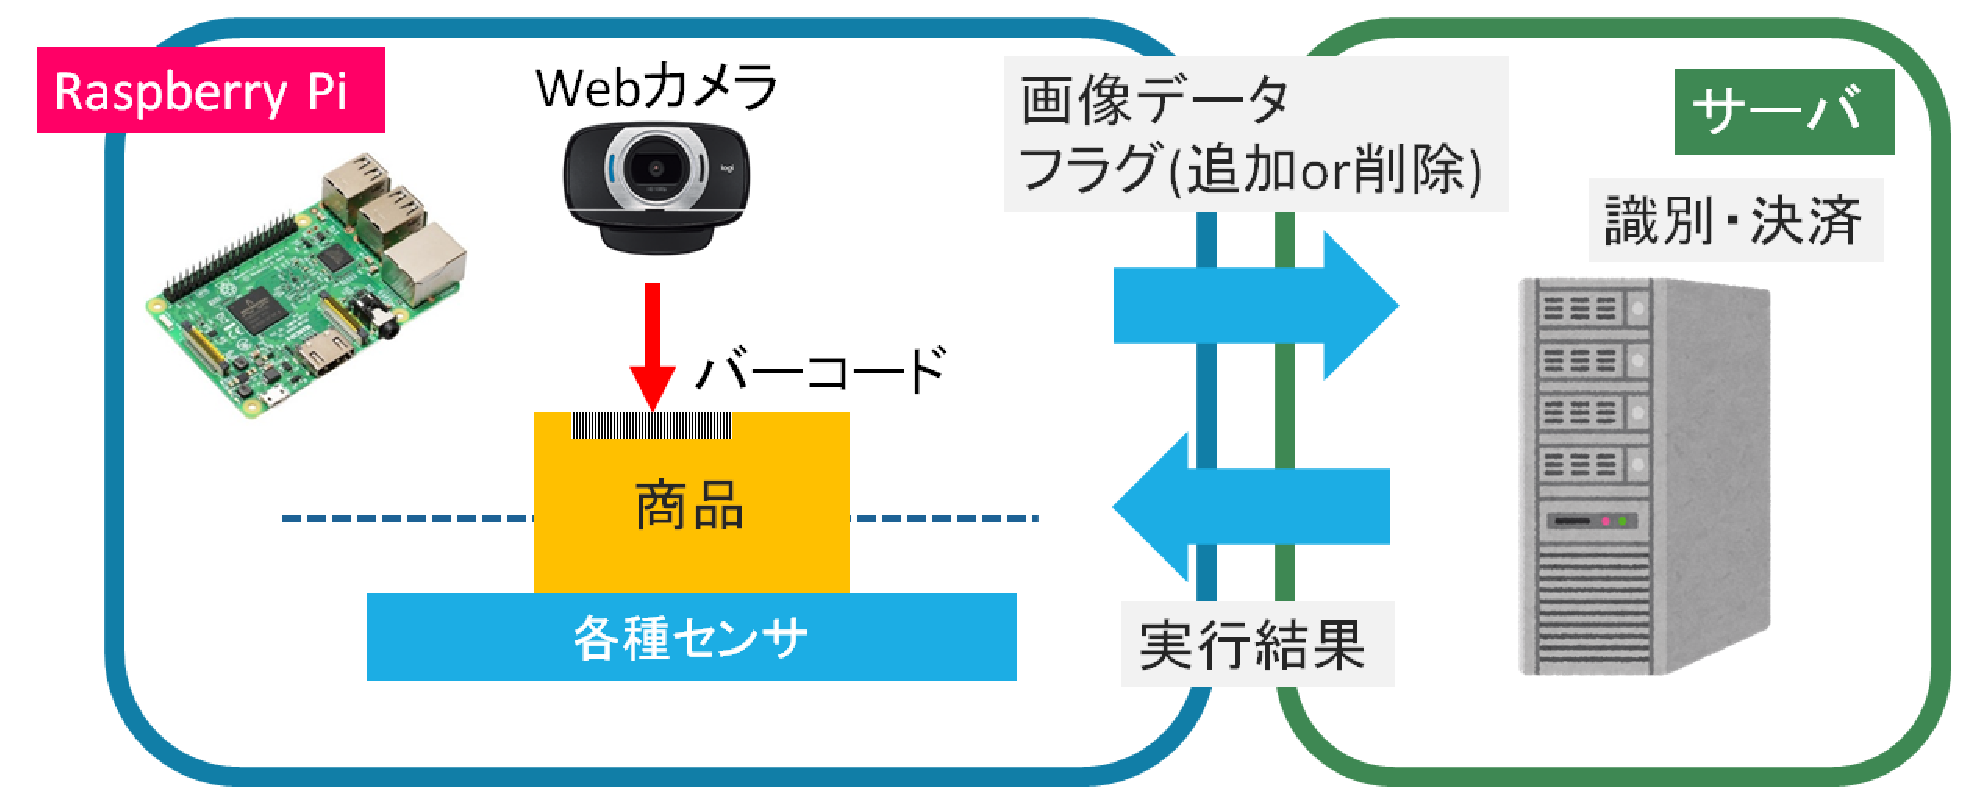
\includegraphics[width = 15cm]{./picture/summary2.eps}
\caption{商品識別システムのイメージ図}
\label{summary2}
\end{figure}


商品識別システムは識別・決済等を行うサーバ側,Raspberry PiとWebカメラ,各種センサを設置した買い物カゴであるRaspberry Pi側の2つのパートで構成される.商品を各種センサが検知した際,Webカメラで商品のバーコードを撮影し,画像データ等をサーバへ送信する.サーバでは商品のバーコード情報等を識別し,最終的に決済を行う.実装の際は,サーバ側を段原丞治が,Raspberry Pi側を真鍋樹が担当した.